\documentclass[10pt, xcolor=table]{beamer}

\setbeamertemplate{note page}[default]
%\setbeameroption{hide notes}
\setbeameroption{show only notes}
%\setbeameroption{show notes}
\setbeamerfont{footnote}{size=\tiny}

\usetheme[progressbar=frametitle]{metropolis}
\usepackage{appendixnumberbeamer}

\usepackage{booktabs}
\usepackage[scale=2]{ccicons}

\usepackage{pgfplots}
\usepgfplotslibrary{dateplot}
\usepackage{multicol}
\setlength{\columnsep}{1.5cm}
\usepackage{multirow}

\usepackage{hyperref}
%\usepackage{animate}
\usepackage{lmodern}
\usepackage[T1]{fontenc}
\usepackage{mathtools}
\usepackage{graphicx}
\usepackage[font=scriptsize]{caption}
\usepackage{tikz}
\usepackage{stackengine}
\usepackage{array}
\usetikzlibrary{positioning}
\usepackage{tabularx}
\usepackage{tabulary}
%\hypersetup{
%    colorlinks=true,
%    linktoc=none,
%    linkcolor=blue,
%    urlcolor=blue
%}

\usepackage[math]{cellspace}
\cellspacetoplimit 2pt
\cellspacebottomlimit 2pt


%\definecolor{set1}{RGB}{228, 26, 28}
%\definecolor{set2}{RGB}{77, 175, 74}
%\definecolor{set3}{RGB}{255, 127, 0}
%\definecolor{set4}{RGB}{166, 86, 40}
%\definecolor{set5}{RGB}{153, 153, 153}

\usepackage{xspace}
\newcommand{\themename}{\textbf{\textsc{metropolis}}\xspace}

\newcommand\Fontvi{\fontsize{8}{9}\selectfont}
\newcommand\Fontvr{\fontsize{6}{7}\selectfont}

\setbeamerfont{parent A}{size=\small}

\DeclarePairedDelimiter\abs{\lvert}{\rvert}%
\DeclarePairedDelimiter\norm{\lVert}{\rVert}%
\makeatletter
\let\oldabs\abs
\def\abs{\@ifstar{\oldabs}{\oldabs*}}
\let\oldnorm\norm
\def\norm{\@ifstar{\oldnorm}{\oldnorm*}}
\makeatother
\newcommand*{\Value}{\frac{1}{2}x^2}%

\newcommand{\floatfootnote}[1]{\ifx\[$\else\footnote{#1}\fi}
\newcommand{\floatfootnotes}[1]{\ifx\[$\else\footnote{#1}\fi}



\title{Digital Transformation of Healthcare}
\subtitle{Study Design and Data Collection}
% \date{\today}
\date{}
\author{Michoel Snow, M.D. Ph.D., Glen Ferguson, Ph.D.}
\institute{Center for Health Data Innovations}
% \titlegraphic{\hfill\includegraphics[height=1.5cm]{logo.pdf}}

\begin{document}

\maketitle

\begin{frame}{Study Design and Data Collection}
	After this lecture students will be able to 
	\begin{itemize}
		\item Assess the quality of data
		\item Trace the steps where data quality can be affected 
		\item Define measures to ensure quality assurance and quality control of data 
		\item Describe the components of an ETL pipeline
		\item Examine data for problems and discuss possible causes
		\item Design a process for imputation of missing data 
	\end{itemize}
\end{frame}


\begin{frame}{Bioinformatics Pipeline}
	\begin{center}
		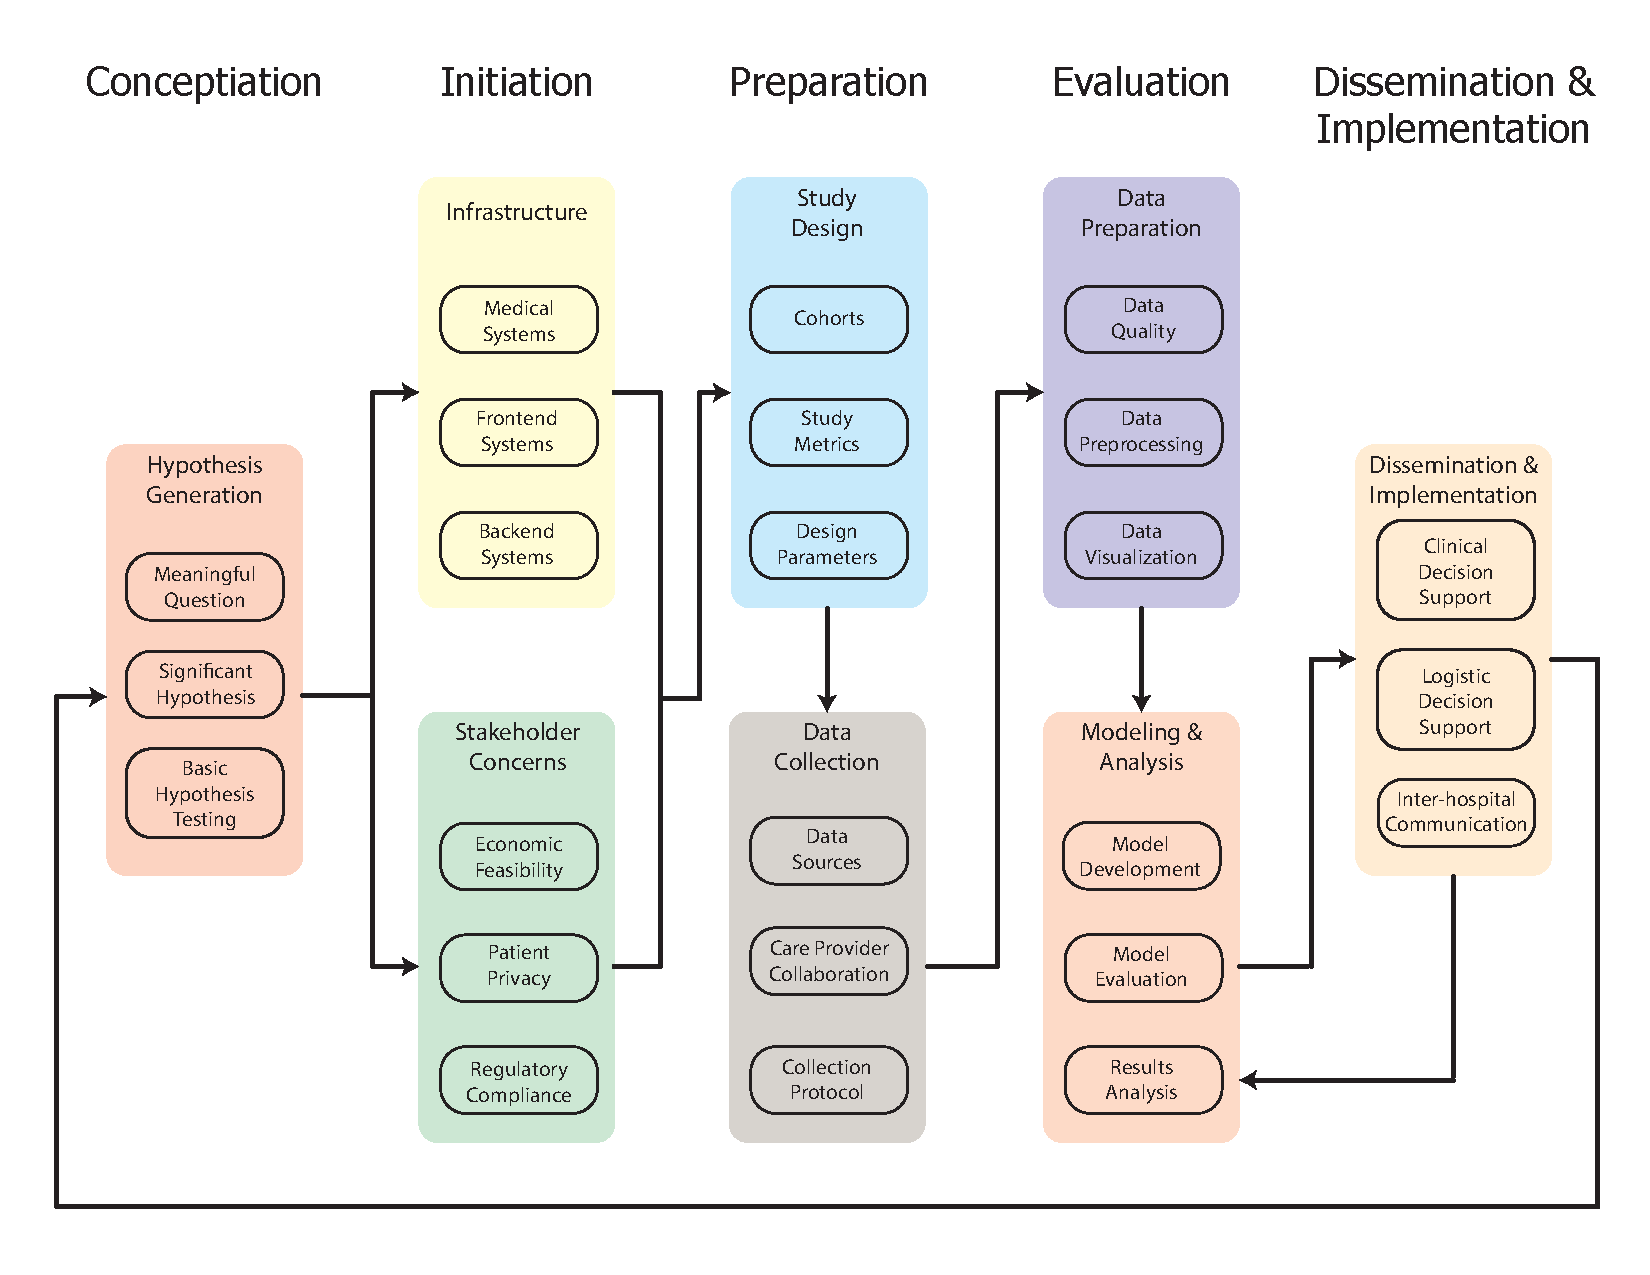
\includegraphics[width=0.9\textwidth]{images/informatics_pipeline.pdf}	
	\end{center}
\end{frame}


\begin{frame}{Study Design and Data Collection}
	\begin{center}
		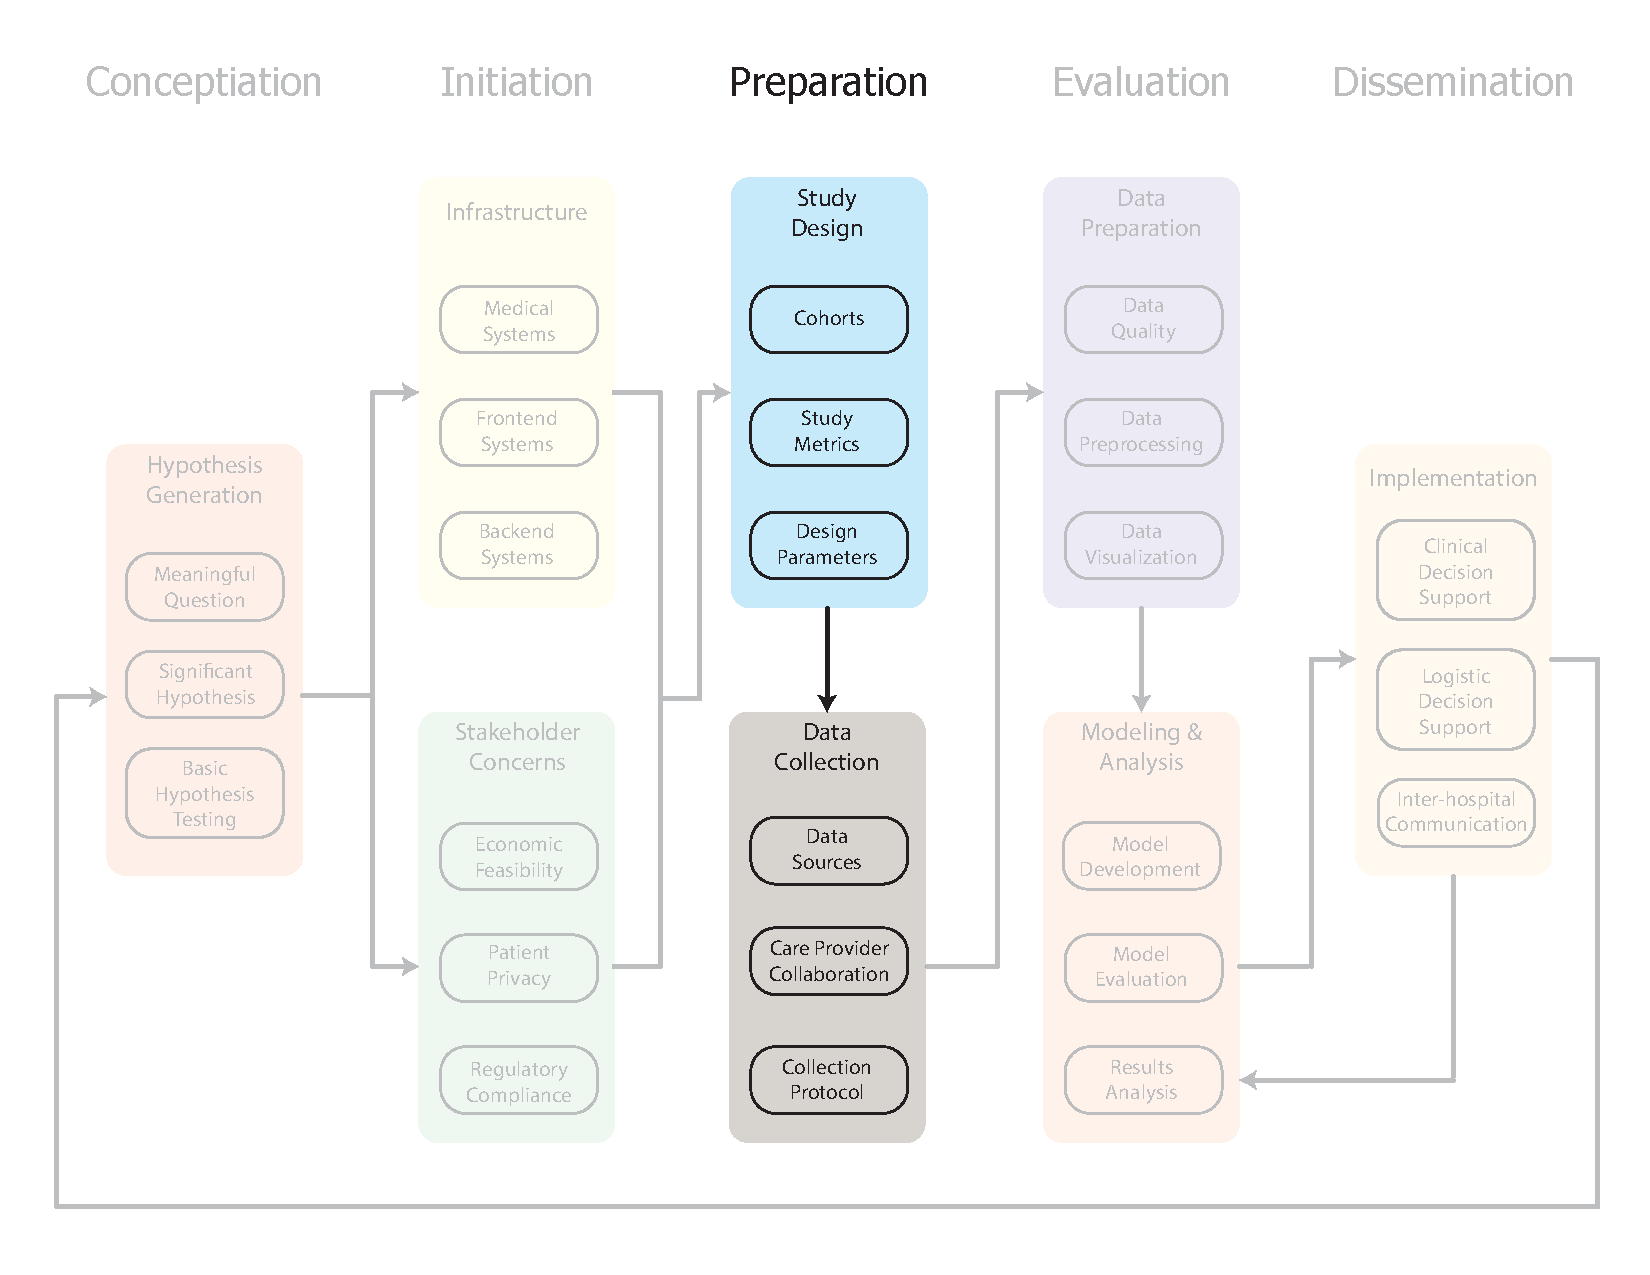
\includegraphics[width=0.9\textwidth]{images/informatics_pipeline_design_collection.pdf}	
	\end{center}
\end{frame}

\begin{frame}{Ancillary Data Sources}
	\begin{itemize}[<+(0)->]
		\item What other kinds of data can be useful to a study (in addition to those generated by the hospital)?
		\item What are the different ways to get that data?
	\end{itemize}
\end{frame}


\note{
\scriptsize
	\begin{itemize}
		\item Other Data - Weather data, public health records 
		\item Try to find that data live (csv, api, scraping), can you trust the data source?
		\begin{itemize}	
			\scriptsize
			\item Weather - download data, weather underground, wunderweather
			\item Twitter - api
			\item football - scraping (ethics of scraping)
			\item Other - ilinet (flu view) pdfs (new york state influenza surveillance)
		\end{itemize}
	\end{itemize}

}



\begin{frame}{Mobile Health Overview }
	\begin{itemize}[<+(0)->]
		\item What devices can we use?
		\item What information can we get from patients, using these devices?
		\item What information should we get from a moral standpoint?
		\item What information do we want and how often do we want it?
	\end{itemize}
\end{frame}

\note{
\scriptsize
	\begin{itemize}
		\item Phones, computers/internet, alexa/google home, smart watches
		\item passive vs active data collections
	\end{itemize}

}

\begin{frame}{mHealth Usability}
	\begin{itemize}
		\item What elements do you have to consider when designing mHealth applications? 
		\item What are the technical (backend) issues?
	\end{itemize}
\end{frame}

\note{
	\scriptsize
	\begin{itemize}
		\item Some of the main components of usability are - learnability, efficiency/speed, memorability, low error rate, satisfaction	
		\item interoperability, data security, confidentiality, integration with current health care systems
	\end{itemize}
}



\end{document}